% vim: set tw=80 aw sw=2 sts=2 noet:
\documentclass{beamer}

%\includeonlyframes{c} % speeding up compilation speed during debug


\usepackage[utf8x]{inputenc}            % diacritice
\usepackage[english]{babel}
\usepackage{color}                      % highlight
\usepackage{alltt}                      % highlight}        % \url{http://...} | \href{http://...}{Nume Link}

% Pentru a include cod decomentati urmatoarele 3 linii
%\usepackage{color}			 % highlight
%\usepackage{alltt}			 % highlight
%\usepackage{code/highlight}	 % highlight

\mode<presentation>
%\usetheme{UEA}
%\usepackage{imperial-beamer}
\usetheme{SCS}

% Pentru a afisa (cont.) la slide-uri prea lungi split-uite pe mai multe pag
\setbeamertemplate{frametitle continuation}[from second]
% Pentru a modifica modul de afisare al numerelor de slide
\setbeamertemplate{footline}[frame number]
\setbeamertemplate{caption}[numbered]

\title[]{Formation Flight for Unmanned Aerial Vehicles}
\subtitle{Bachelor Thesis: July 10\textsuperscript{th},  2013}
\institute[CS]{Prof. Adina Magda Florea \newline Ing. Mihai Trăscău \newline Ș.l. Cătălin Leordeanu}
\author[A]{Alexandru George Burghelea \newline \textit{aburghelea@rosedu.org}}

\begin{document}

{
  % Schimbam fundalul aici pentru a avea slide-ul cu logo-urile
  % Nu știu momentan cum se face asta în template.
  \usebackgroundtemplate{
\includegraphics[width=\paperwidth]{title}}
  \frame{\titlepage}
}

\begin{frame}{Presentation Layout}
  \begin{itemize}
    \item Domain
    \item Autonomous UAV
    \item Hirrus
    \item Platform Objectives
    \item Platform Simulation Architecture
    \item Autopilot Architecture
    \item Thesis Objectives
    \item Formation Flight
    \item Types of Formation
    \item Tested Formations
    \item Evaluation and Results
    \item Conclusions and Future Work
\end{itemize}
\end{frame}

% 1 Slide titlu
% 1 Slide cuprins
% - Domeniu (2-3 slide-uri) ce inseamna uav, ce ar tb sa faca o flota de uav- hirrus 1 slide
% - autonomus uav (colaborare cu TNI)
% obiective, poza arhitectura
% - Zbor in formatie (motivatie) de ce + scenarii
% - descriu formatia
% - care e sistemul de coordonate (putine detalii)
% - formatiile tratate
% 2 slide-uri rezumat rezultate

\begin{frame}{Unmanned Aerial Vehicle}
\textbf{UAV} (\textit{Unmanned Aerial Vehicle})
\begin{tabular}{l l}
\begin{minipage}{0.5\textwidth}
\begin{itemize}
\item no pilot \textbf{on board}
\item remote controlled or
\item completely autonomous
\item envisioned by N. Tesla in 1915
\item used in military and civil missions
\item rotor based or fixed-winged
\end{itemize}
\end{minipage}
&
\begin{minipage}{0.5\textwidth}
\begin{figure}[p]
\includegraphics[width=2in]{img/uav1.jpg}
\caption{Fixed-wing UAV with surmountable camera [1]}
\end{figure}
\end{minipage}
\end{tabular}

\end{frame}

\begin{frame}{Autonomous UAV}
About:
\begin{itemize}
\item in collaboration with \textit{Teamnet International S.A.}
\item aims to build a management platform for a fleet of UAVs
\end{itemize}
Objectives:
\begin{itemize}
\item development of an autonomous flight software agent embedded on Raspberry PI
for Hirrus
\item development of a software platform for programming, monitoring and autonomous mission deployment for UAVs
\end{itemize}
\end{frame}

\begin{frame}{Platform Objectives}
\begin{itemize}
\item Ground Control System (based on QGroundControl)
\item Mission Monitoring System
\item Adding \textit{collision avoidance} and \textit{formation flight} capabilities to the Hirrus Autopilot
\item Designing and implementing an embedded AI software agent responsible for mission management (re)planning and execution
\end{itemize}
\end{frame}

\begin{frame}{Hirrus}
\begin{center}
\begin{figure}[p]
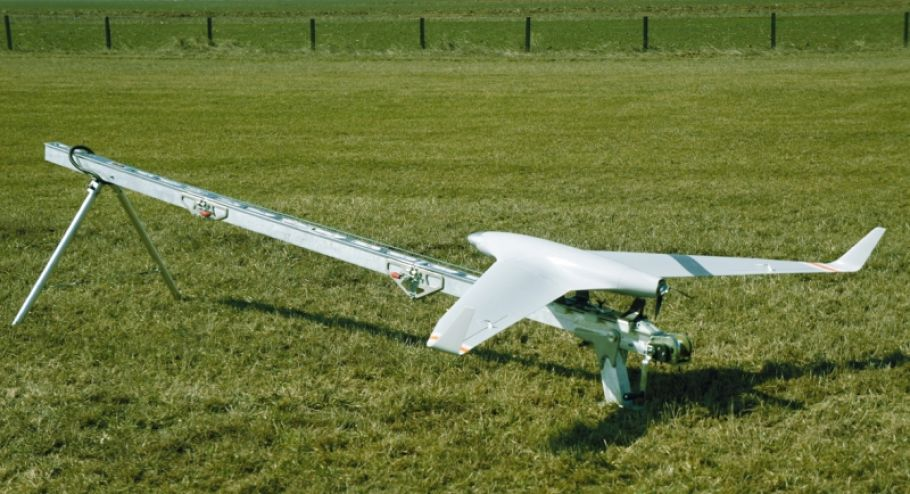
\includegraphics[width=3.5in]{img/hirrus.jpg}
\caption{Hirrus UAV [2]}
\end{figure}
\end{center}
\end{frame}

\begin{frame}{Hirrus}

\begin{description}
\item [Destination] law enforcement, reconnaissance, search and rescue, cartography
\item [Dimensions] Wingspan 2.35 m / Length 1.1 m / Weight 7 kg
\item [Speed] Max 130 km/h, Cruise 90 km/h
\item [Payload] 0.7 kg
\item [Propulsion] Electric
\item [Endurance] 180 min
\item [Range] 15 km
\end{description}

\end{frame}

\begin{frame}{Used Technologies}
\begin{tabular}{l l}
\begin{minipage}{0.5\textwidth}

\begin{figure}
\begin{itemize}
\item simulated using Rascall Drone
\end{itemize}
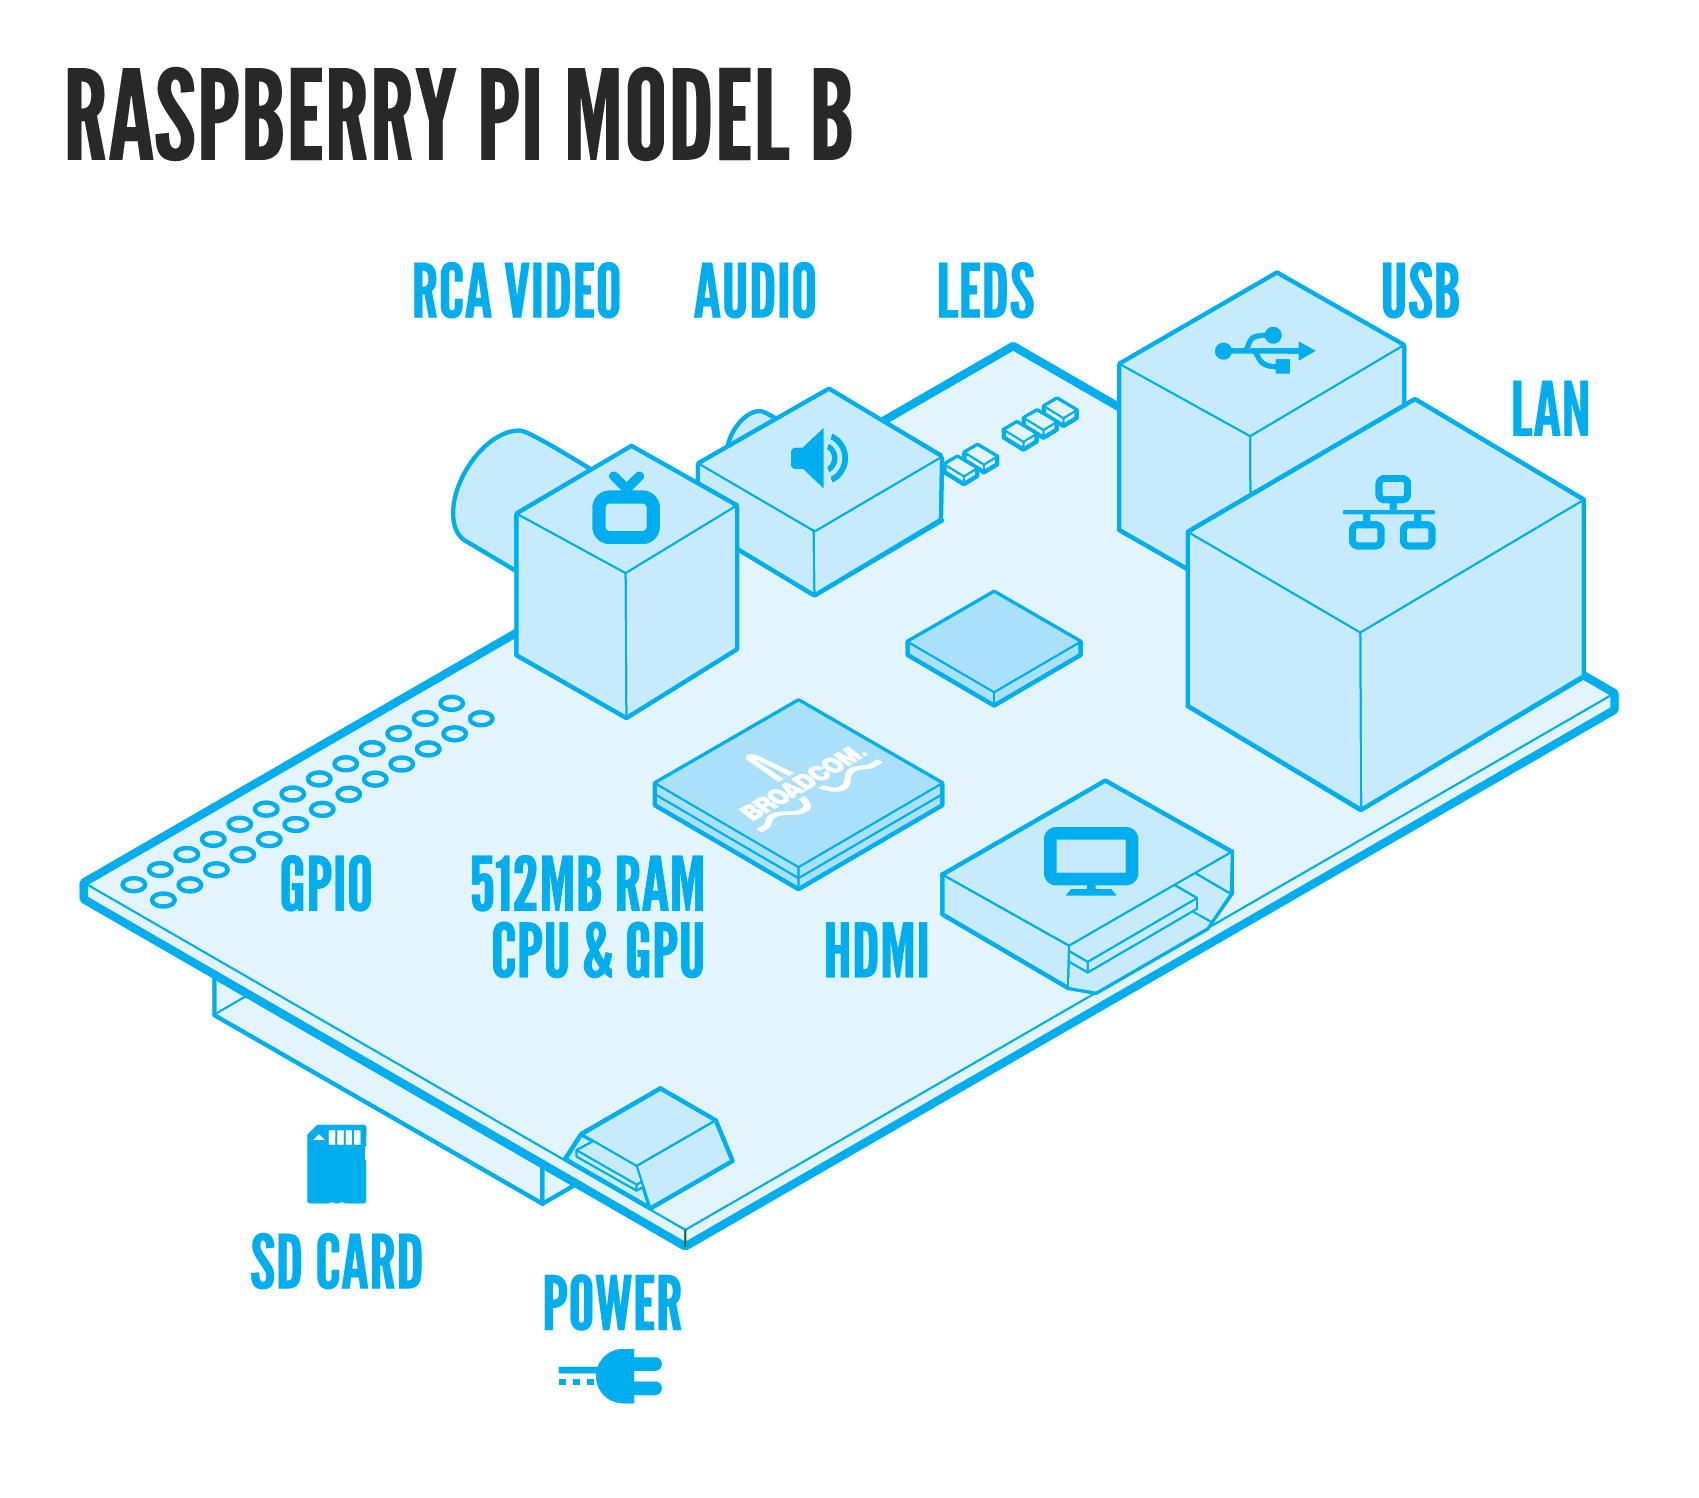
\includegraphics[width=1in]{img/rpi.png}
\caption{Raspberry PI}
\end{figure}
\end{minipage}
&
\begin{minipage}{0.5\textwidth}
\begin{figure}

\includegraphics[width=1in]{img/fglogo.png}
\caption{Flight Gear Flight Simulator}

\includegraphics[width=1.5in]{img/qgclogo.png}
\caption{QGroundControl}
\end{figure}
\end{minipage}
\end{tabular}
\end{frame}

\begin{frame}{Platform Simulation Architecture}

\begin{center}
\begin{figure}[p]
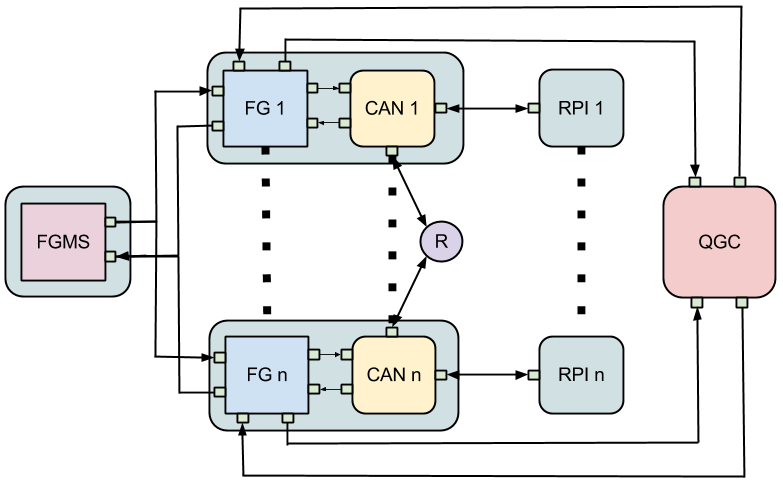
\includegraphics[width=\textwidth]{img/platform-architecture.png}
\caption{Platform Architecture}
\end{figure}
\end{center}
\end{frame}

\begin{frame}{Embedded Software Agent Architecture}
\begin{center}
\begin{figure}[p]
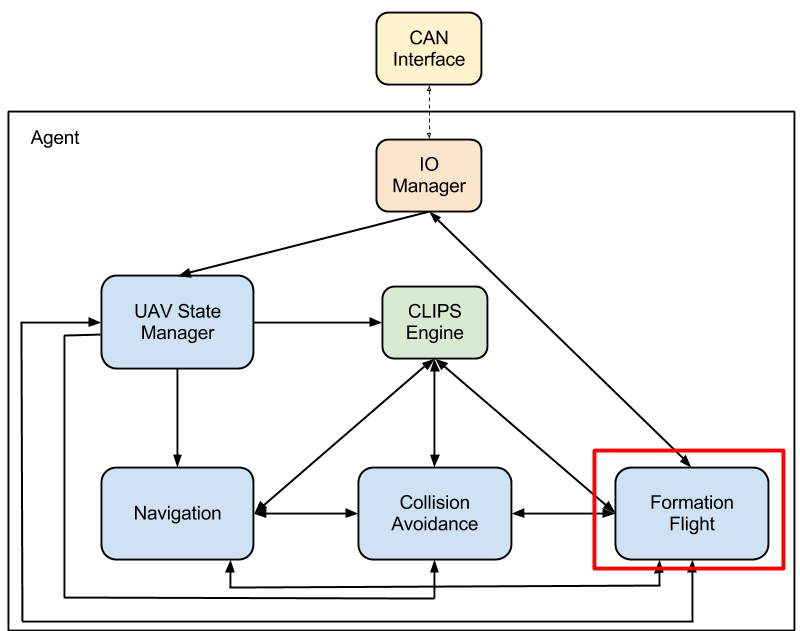
\includegraphics[width=3in]{img/rpi-architecture.png}
\caption{Embedded Software Agent Architecture}
\end{figure}
\end{center}
\end{frame}

\begin{frame}{Thesis Objectives}
\begin{itemize}
\item close range formation flight module
\item using decentralized communication
\item multi agent system with reactive agents inspired by swarm structures and behavior models
\item 3 or more UAVs flying in formation
\item drones flying at close range
\end{itemize}
\end{frame}

% \begin{frame}{Formation Flight}
% \begin{itemize}
% \item simulated using Flight Gear Flight Simulator
% \item follow the leader behavior
% \item GPS and ECEF coordinates based on WSG84 ellipsoid
% \end{itemize}
% \end{frame}

\begin{frame}{Formation Types}
\begin{center}
\begin{figure}[p]
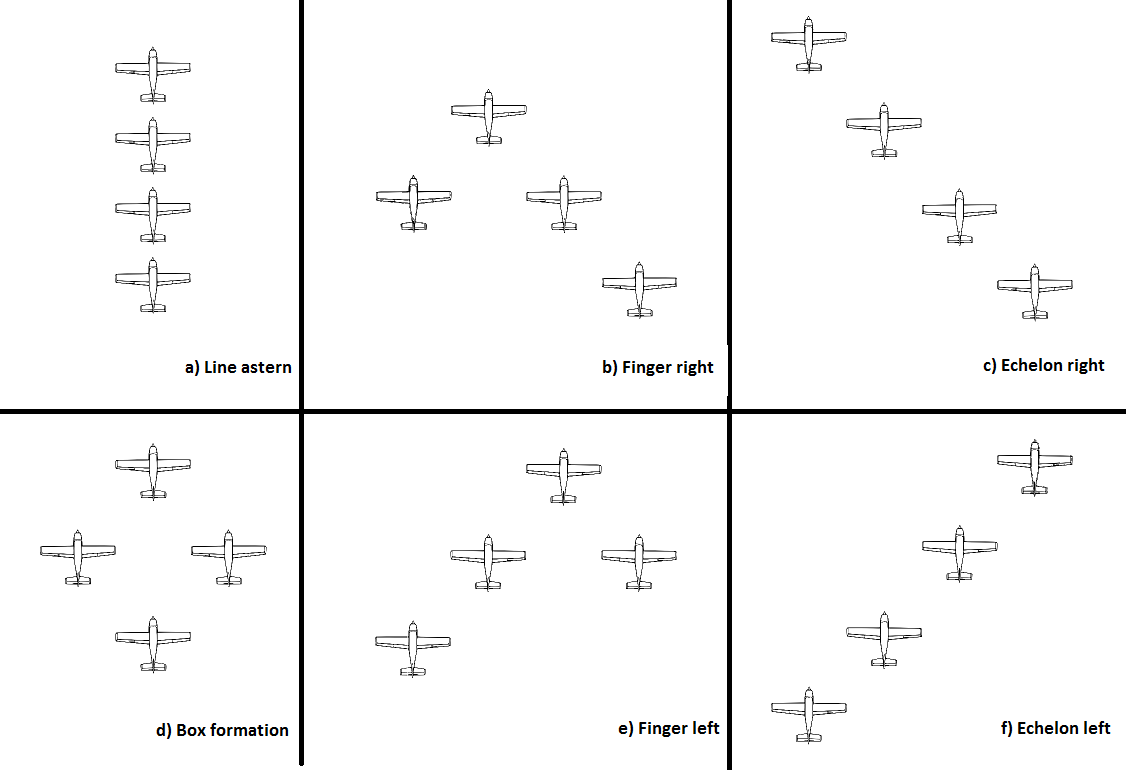
\includegraphics[width=3.5in]{img/4form.png}
\caption {Formation Types}
\end{figure}
\end{center}
\end{frame}

\begin{frame}{Tested Formations}
% 
% \begin{tabular}{l l}
% \begin{minipage}{0.5\textwidth}
% 3 UAVs Formations
% \begin{itemize}
% \item{Line Astern}
% \item{V Formation}
% \end{itemize}\end{minipage}
% &
% \begin{minipage}{0.5\textwidth}
\begin{figure}[p]
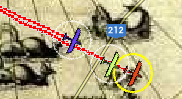
\includegraphics[width=1.6in]{img/lqgc.png}
\caption{Top view of Line Astern}
\end{figure}
\begin{figure}[p]
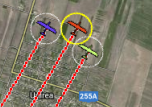
\includegraphics[width=1.6in]{img/vqgc.png}
\caption{Top view of V Formation}
\end{figure}
% \end{minipage}
% \end{tabular}
\end{frame}



\begin{frame}{Implementation details}
\begin{itemize}
\item follow the leader behavior
\item GPS and ECEF coordinates based on WSG84 ellipsoid
\item \textit{variable matching behavior} for formation maintaining
\item \textit{follow behavior} for entering formation
\item C++ with Boost library code base
\end{itemize}
\end{frame}

\begin{frame}{Evaluation and Results}
\begin{itemize}
\item tested with dedicated leader
\item leader with predefine mission
\item other UAVs have a \textit{follow the leader} behavior
\item communication delay increases probability of breaking formation and increases efforts for formation maintaining
\item 300 feet ( $<100$ m) distance between UAVs
\item for closer formations a more robust coordinate system is needed
\item computational errors are induced by the ellipsoid model while converting coordinates
% \item 9\% to 25\% of time spend for maintaining the formation
% \item 60\% to 70\% of time spend for entering the formation
% \item 15\% to 20\% of time relieving control for collision avoidance
% \item communication delay increases probability of breaking formation and increases efforts for formation maintaining
% \item 300 feet ( $<100$ m) distance between UAVs
% \item for closer formations another coordinate system is needed
% \item computational errors are induced by the ellipsoid model while converting coordinates
\end{itemize}
\end{frame}

\begin{frame}{Evaluation and Results}
\begin{center}
\begin{figure}[p]
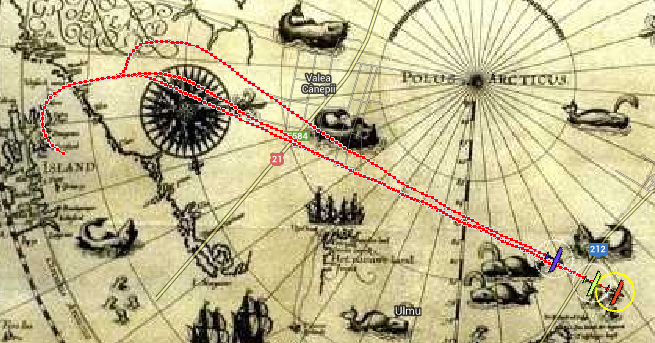
\includegraphics[width=4in]{img/lineastern.png}
\caption{QGroundControl flight path for Line Astern simulation}
\end{figure}
\end{center}
\end{frame}

\begin{frame}{Evaluation and Results}
\begin{center}
\begin{figure}[p]
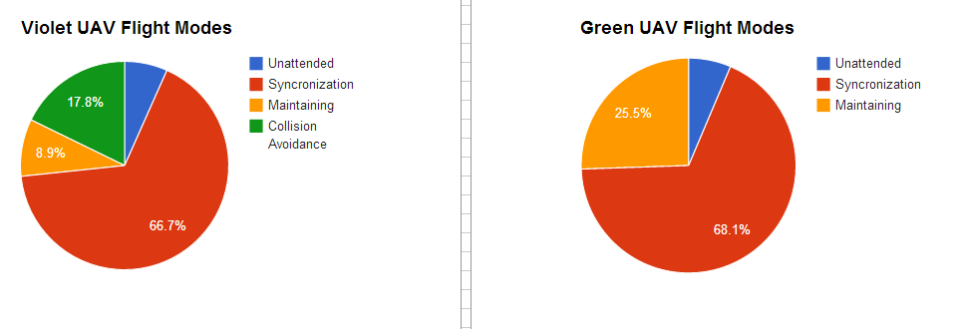
\includegraphics[width=4in]{img/flight-modes.png}
\caption{Time percentage of flight modes usages}
\end{figure}

\end{center}
\end{frame}

\begin{frame}{Conclusions and Future Work}
Conclusions:
\begin{itemize}
\item \textit{Line Astern} and \textit{V Formation}
\item reactive software agent for formation flight
\item decentralized communication
\end{itemize}
Future Work:
\begin{itemize}
\item formations based on a virtual leader (geometrical center of formation)
\item simulating with Flight Gear instances running on dedicated machines
\item communication between Raspberry PI (holding AI software agents) and Hirrus via CAN bus
\item PID controllers for speed and steering
\end{itemize}
\end{frame}

\begin{frame}{References}
\begin{itemize}
\item \textit{[1] http://http://aerosdb.com/uav-drone/}
\item \textit{[2] http://aft.ro/bro.pdf}
\end{itemize}
\end{frame}

\begin{frame}{Questions}
\begin{center}
\fontsize{60}{70}\selectfont Q\&A
\end{center}
% Keywords:
% \begin{itemize}
% \item UAV
% \item Decentralized
% \item Reactive
% \item Flight Gear
% \item Hirrus
% \item QGroundControl
% \item Formations
% \item Communication
% \item Swarm
% \item Close Range Formation
% \end{itemize}
\end{frame}
\end{document}
